\chapter{Estudo 2: Dimensionamento dinâmico da potência alocada na reserva secundária}

\section{Dados Utilizados\label{se:dadosestudo}}

Os dados em estudo são do mercado energético espanol, retirados do site da \href{https://www.esios.ree.es/es}{ESIOS}.


\begin{table}[H]
    \caption{Indicadores retirados do site da ESIOS}    
    \resizebox{\linewidth}{!}{\csvautotabular{tabelas/indicators_metadata.csv}}
\end{table}


\subsection{Aquisição dos Dados}

No ambito da automatização destes dados foi modificado o repositorio \href{https://github.com/SanPen/ESIOS}{ESIOS} para ser usado como uma biblioteca de python, aberta, em pypi.\\
Sendo uma ferramenta mais facilmente acessivel para a extrair dados do mercado espanhol, \href{https://pypi.org/project/pyesios/}{pyesios}. \\
No âmbito de automatizar o processo, foram feitas contribuições a esta ferramenta para tornar mais acessível, e uma ferramenta aberta de python\\


\thispagestyle{plain}

\section{Estudo dos dados}

Os dados que proponho a prever são os de Energia Usada na Banda de Reserva Secundária, tanto a subir como a descer: "UpwardUsedSecondaryReserveEnergy","DownwardUsedSecondaryReserveEnergy".\\



\begin{figure}[H]
  \centering
  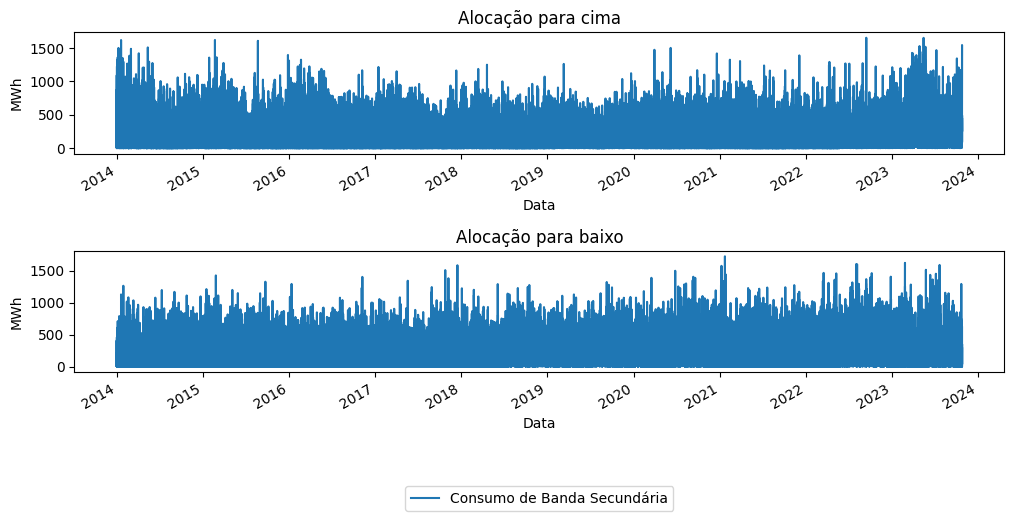
\includegraphics[width=\textwidth]{plots/consumo_originais.png}
  \caption{Serie Temporal dos dados alvo}
  \label{fig:targettimeseries}
\end{figure}


Para termos uma melhor percepção dos mesmos segue algumas janelas temporais mais pequenas.

\begin{figure}[H]
  \centering
  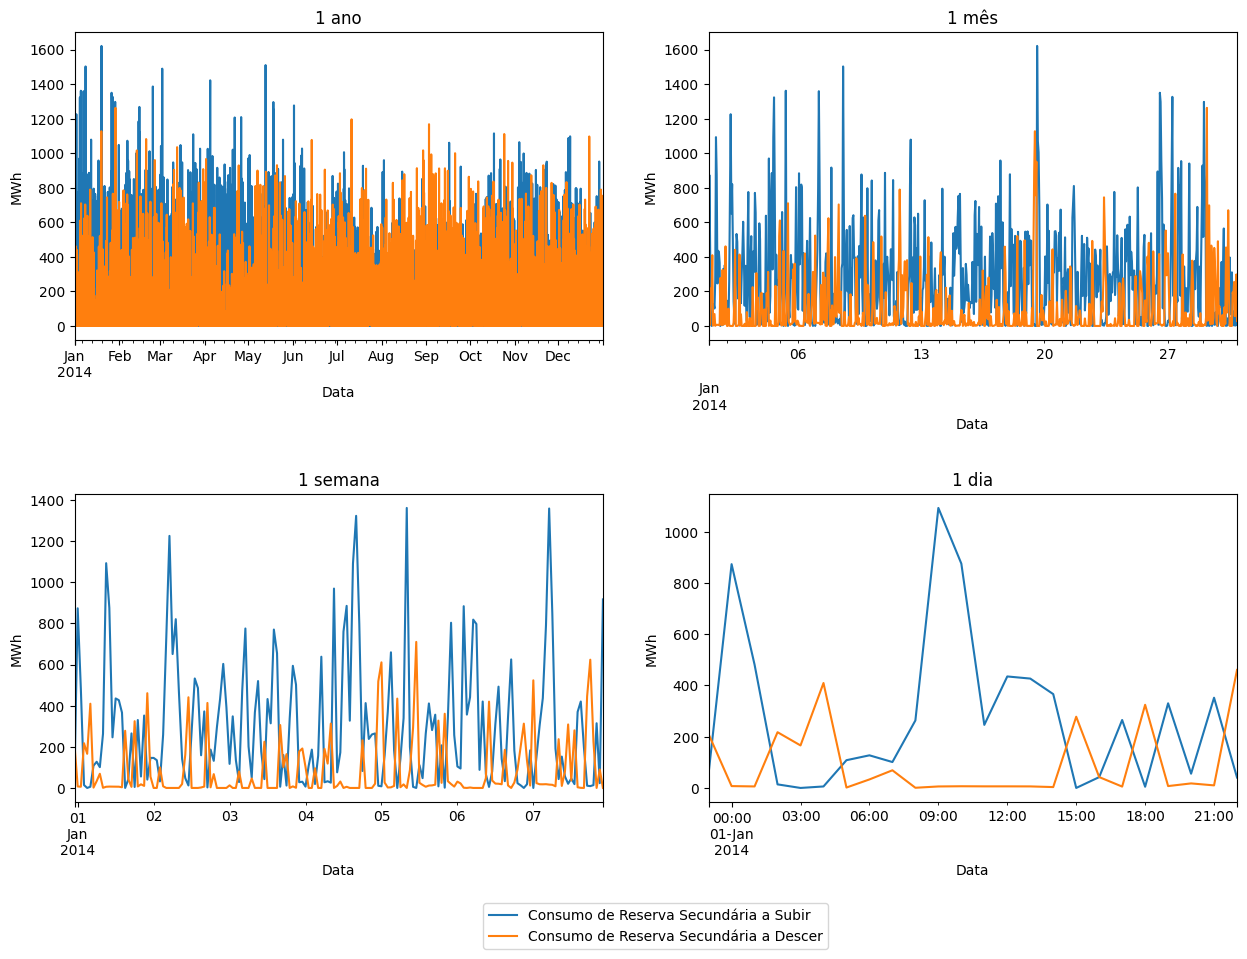
\includegraphics[width=\textwidth]{plots/target_timeseries_windows.png}
  \caption{Janelas Temporais dos dados alvo}
  \label{fig:targettimeserieswindows}
\end{figure}


Estas mostram claramente que ambos os atributos mantêm um comportamento tanto discreto, como linear, isto é, que ou existe algum valor, ou é zero, e se existe valor este tem comportamento linear.\\
A distribuição destes dados é claramente exponencial. O que é importante para a escolha de alguns parâmetros na modelação. \\

		
\begin{figure}[H]
  \centering
  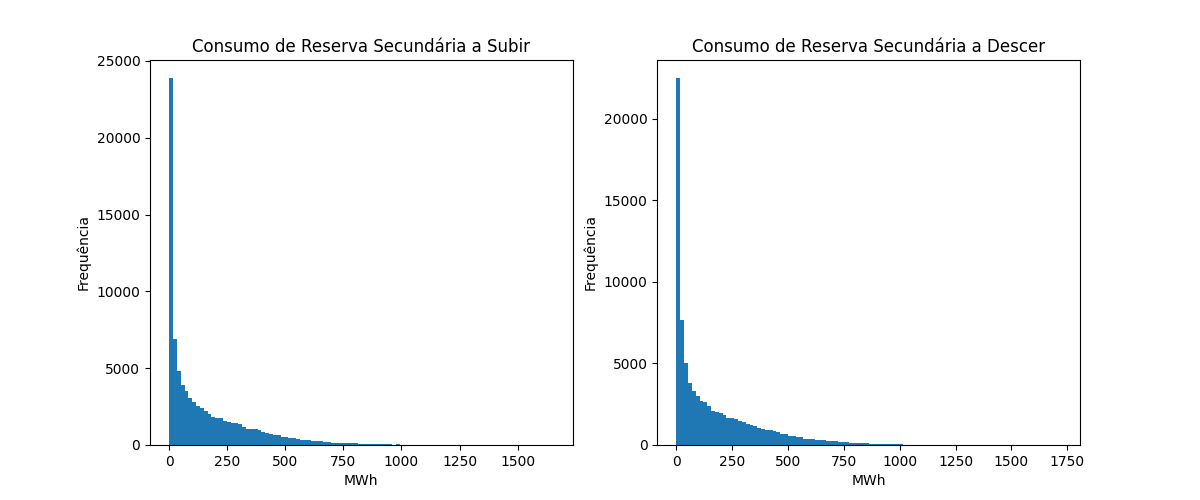
\includegraphics[width=\textwidth]{plots/target_histograms.png}
  \caption{Frequência dos dados alvos}
  \label{fig:targethistograms}
\end{figure}


\subsection{Correlações}

Os modelos vão depender bastante de correlação entre variáveis.

Nesta secção queremos tentar identificar se há visiveis relações entre as variáveis, e se há relações temporais  visiveis nas colunas alvo.


\subsubsection{Correlações entre atributos}


\begin{figure}[H]
  \centering
  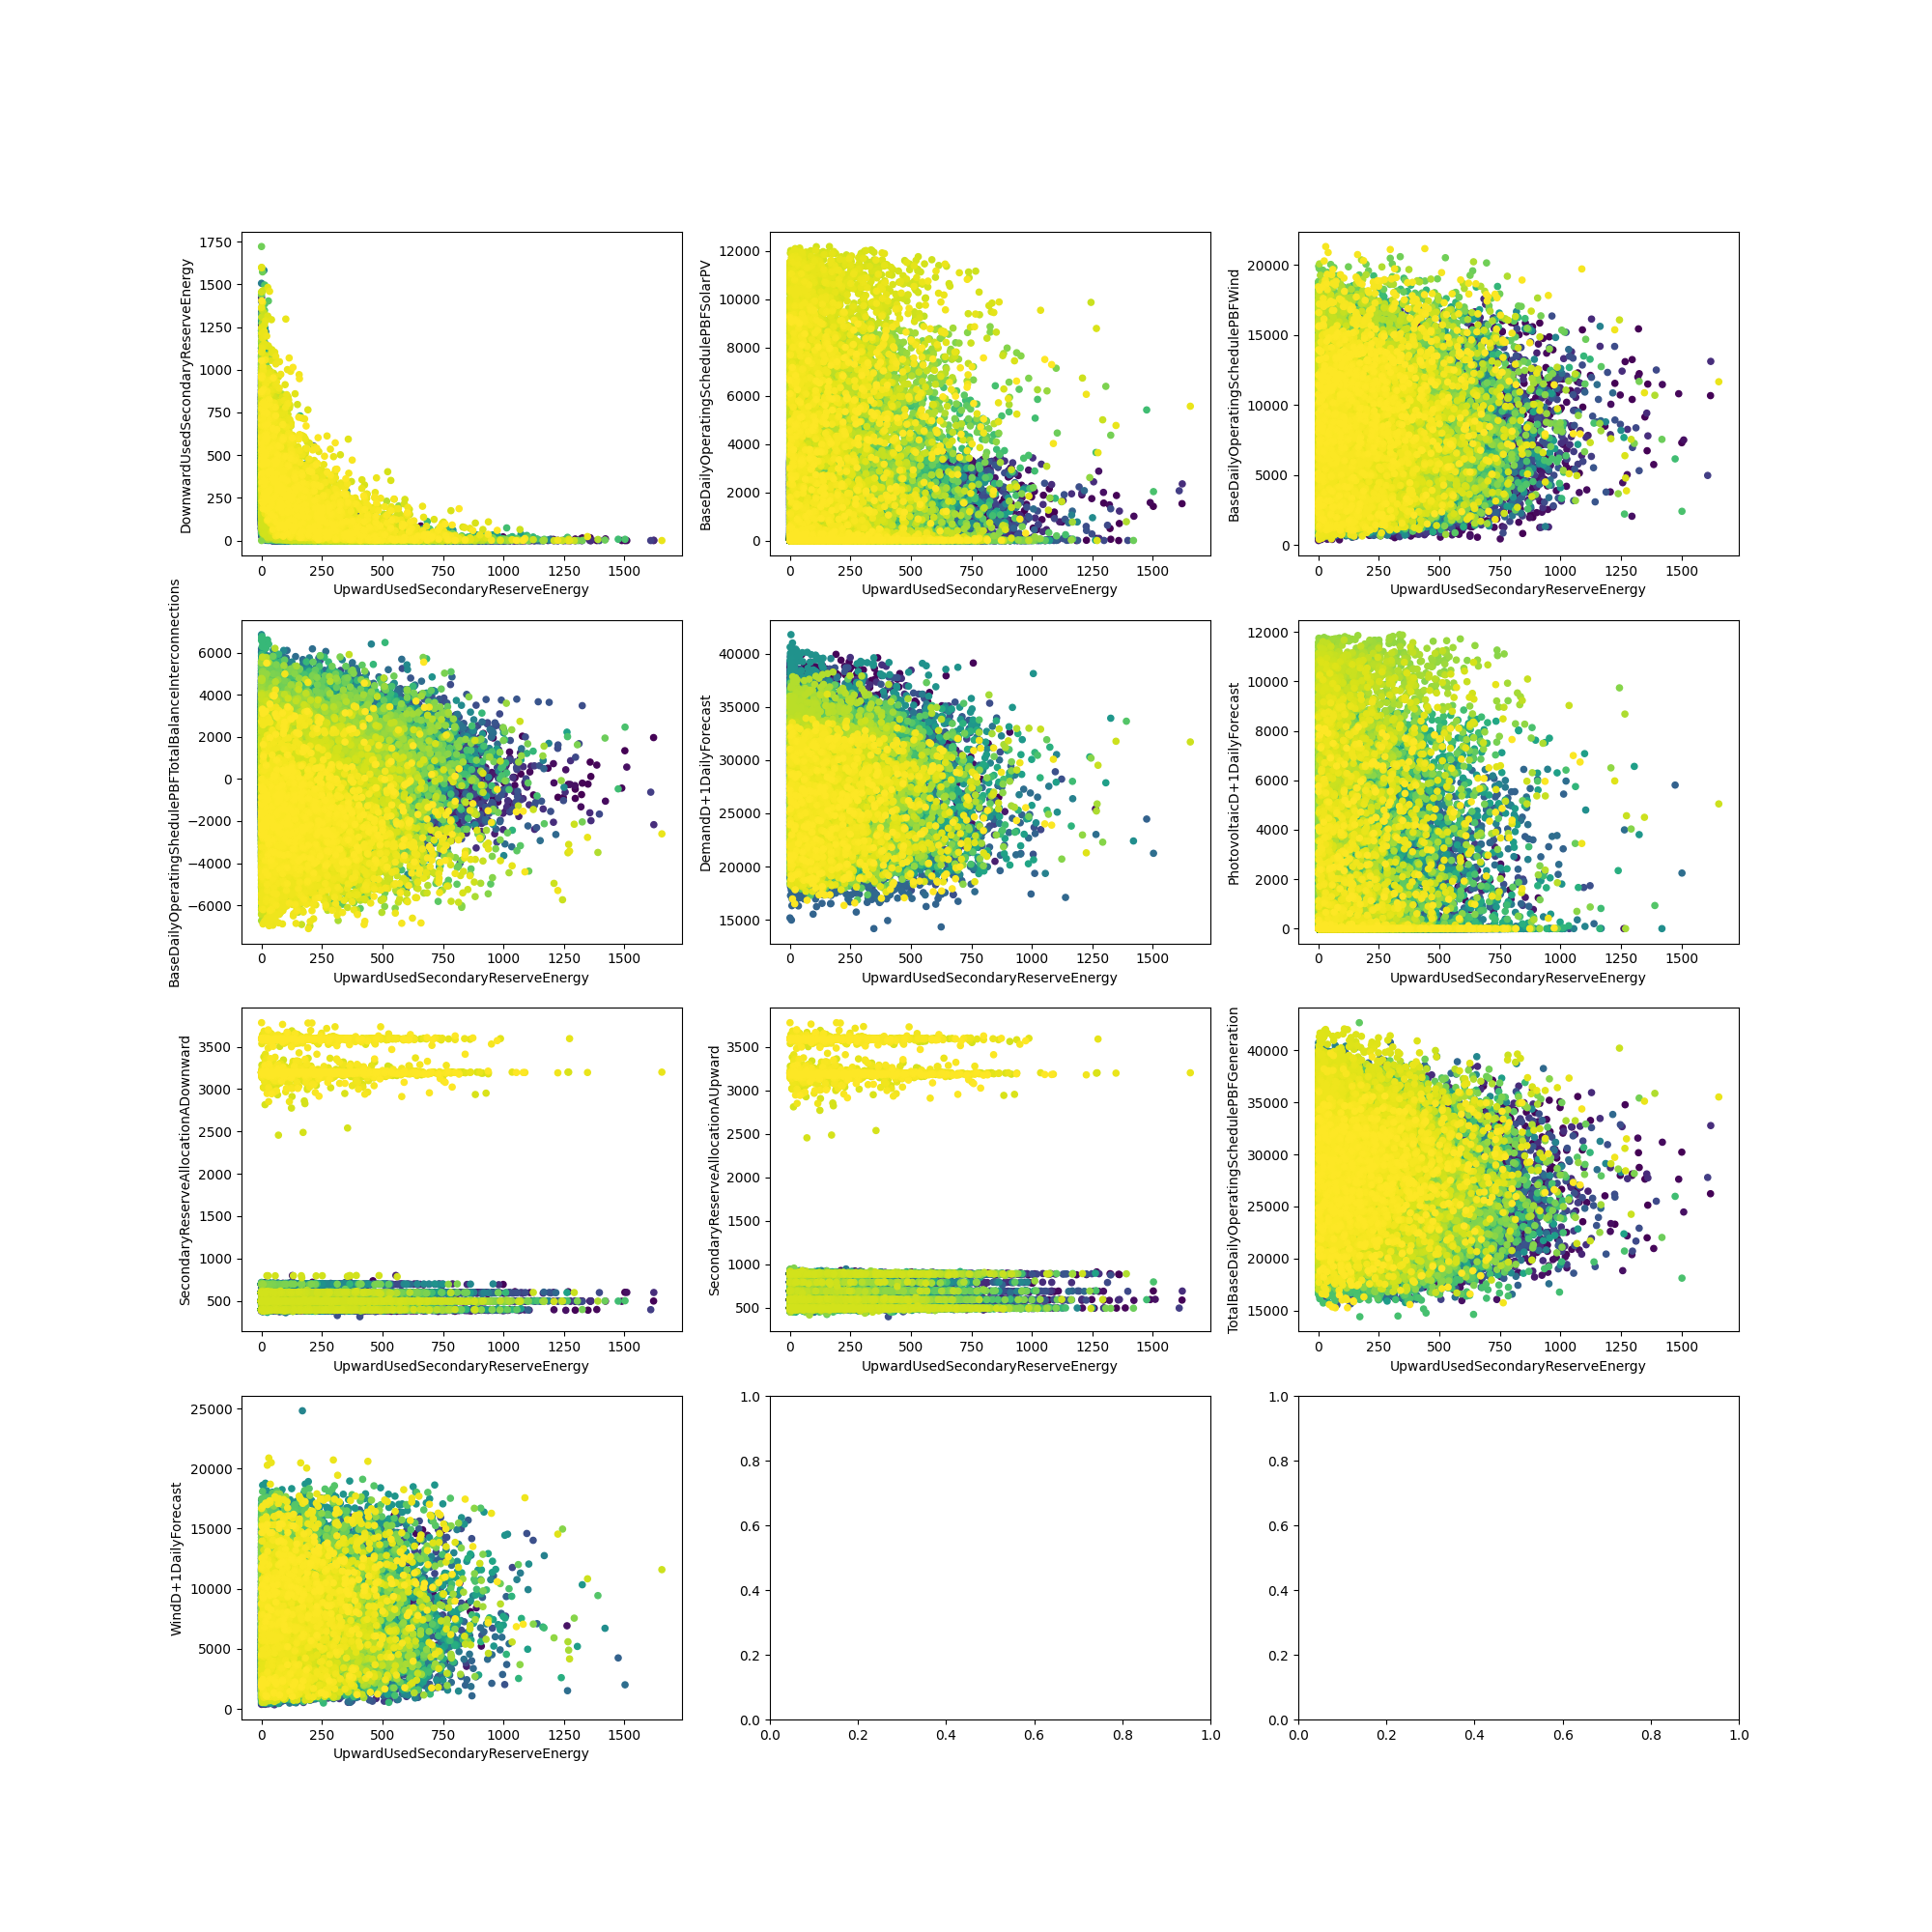
\includegraphics[width=\textwidth]{plots/feature_correlation.png}
  \caption{Correlação entre atributos}
  \label{fig:featurecorrelation}
\end{figure}

Esta figura apresenta a dispersão de valores entre a energia usada, primeiras três linhas a energia para cima e as seguintes a energia para baixo, e os outros atributos presentes.\\
As correlações entre variáveis parecem muitos escassas, o que apresenta já que a previsão destes dados usando estas variáveis vai ser um problema difícil.\\
Por norma é feito uma seleção de atributos baseado nestas correlações, eliminando assim os atributos que ajudam menos, ou até prejudicam os modelos.\\
Segue os valores de correlação onde podemos ver numericamente que existe muito pouca correlação entre os atributos. Onde a primeira coluna são os valores de correlação para a energia usada a subir e a segunda coluna as correlações da energia usada a descer.\\

\begin{figure}[H]
  \centering
  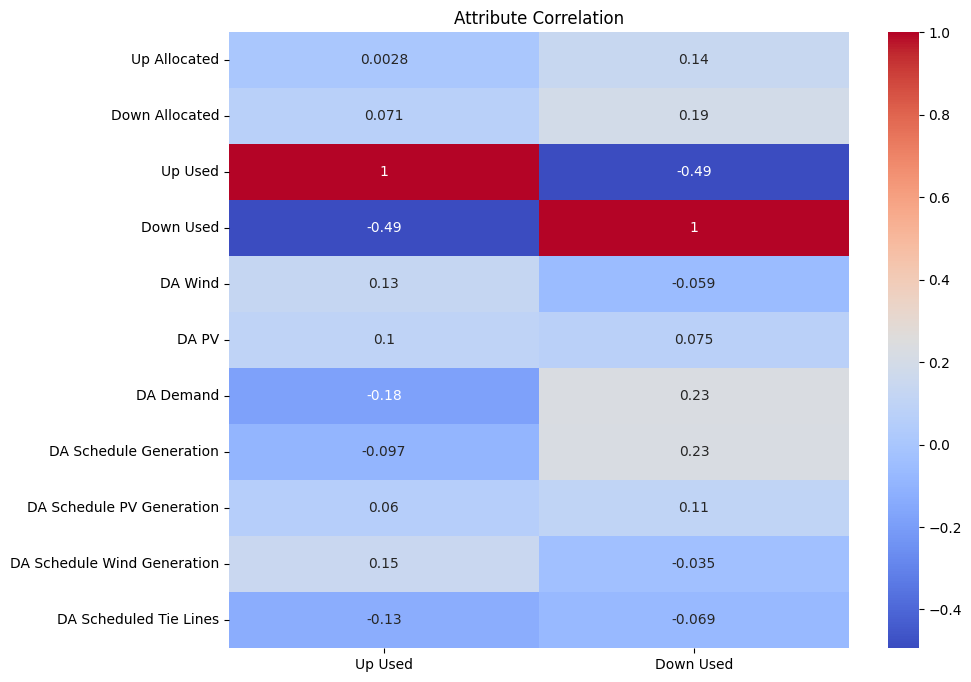
\includegraphics[width=\textwidth]{plots/correlation_heatmap.png}
  \caption{Valores de correlação entre atributos}
  \label{fig:correlationheatmap}
\end{figure}

\subsubsection{Correlações Temporais}

\begin{figure}[H]
  \centering
  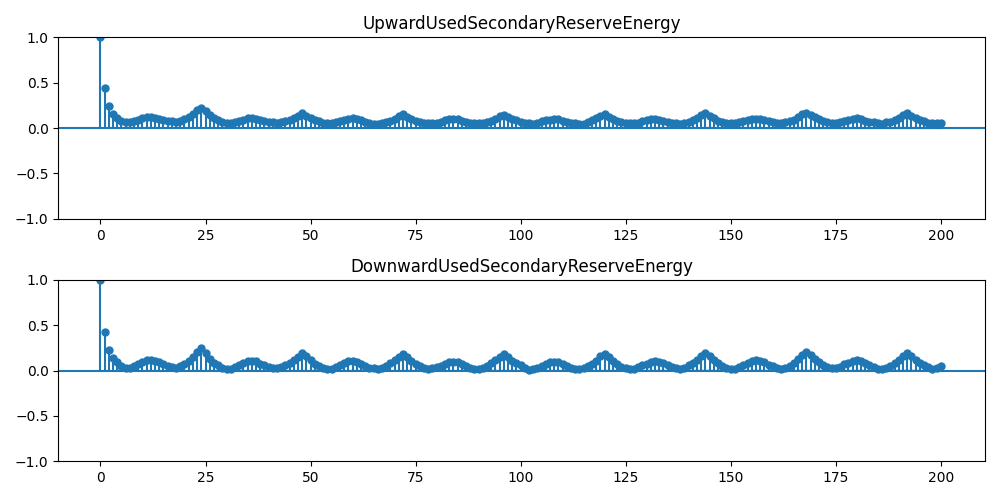
\includegraphics[width=\textwidth]{plots/autocorrelation.png}
  \caption{Autocorrelação Temporal}
  \label{fig:autocorrelation}
\end{figure}

A autocorrelação, em ambos os alvos, é mais forte nas 3 horas mais próximas, e nos pontos com diferença de 12 e 24 horas. \\
É de notar que estes valores são baixos, prometendo já também uma baixa regressividade temporal. \\
Os melhores saltos temporais e suas correlações são mostradas na tabelas em baixo:\\


\begin{table}[H]
  \caption{Autocorrelação Temporal}    
  \resizebox{\linewidth}{!}{\begin{tabular}{lllllllllll}
\toprule
\midrule
\multirow[t]{2}{*}{UpwardUsedSecondaryReserveEnergy} & horas & 1 & 2 & 24 & 23 & 25 & 168 & 144 & 192 & 48 \\
 & rácio & 0.44 & 0.24 & 0.22 & 0.19 & 0.19 & 0.17 & 0.16 & 0.16 & 0.16 \\
\cline{1-11}
\multirow[t]{2}{*}{DownwardUsedSecondaryReserveEnergy} & horas & 1 & 2 & 24 & 23 & 25 & 168 & 144 & 192 & 48 \\
 & rácio & 0.43 & 0.22 & 0.25 & 0.20 & 0.19 & 0.21 & 0.19 & 0.20 & 0.19 \\
\cline{1-11}
\bottomrule
\end{tabular}
}
  \label{tab:tempcorr}
  \end{table}

Outro ponto a denotar é que os objectos não têm um comportamento completamente linear, i.e., parece existir um comportamento discreto na questão ser alocado ou não esta reservas secundárias, e caso seja alocado, aí existir alguma linearidade. \\
Logo qualquer tipo de modelação terá de resolver primeiramente este problema. \\
Estas relações mostram que em termos de atributos usados vai ser um desafio complicado para qualquer tipo de modelo. \\
No âmbito desta dissertação queremos verificar a qualidade das previsões usando estes mesmo atributos, logo, não será feita seleção dos mesmos. \\
A nível da relação temporal, a maior parte dos modelos que iremos testar aplica um janela na dimensão temporal, usando todos os valores nessa janela, e aplicando os pesos nessas distâncias que mais se enquadram. Logo também não é relevante escolher apenas as distâncias temporais com maior correlação, pois os modelos vão fazer essa pesagem. \\


 \label{se:dadoscrus}



\thispagestyle{plain}



\section{Tratamento dos dados}

\textbf{Normalização} \par
A normalização foi deixada por ser aprendida nos modelos, sendo que todos têm como segunda camada, uma de normalização.\par

\textbf{Limpeza} \par

Podemos ver pelos gráficos seguintes que a existem alguns outliers, sendo estes definidos como 3 desvios padrão de distância à média.\par
Estes gráficos mostram também que existe uma variação do que são os valores normais de cada atributo a nível temporal. Logo um método de limpeza não se poderia basear apenas numa definição geral de outliers, mas teria de ser feito em janelas temporais.\par
Pelo mesmo argumento e visto que os outliers fazem parte do que queremos também descobrir, não é aplicada nenhum método de remoção dos mesmo, sendo os dados passados a cru para os modelos.\par


\begin{figure}[H]
  \centering
  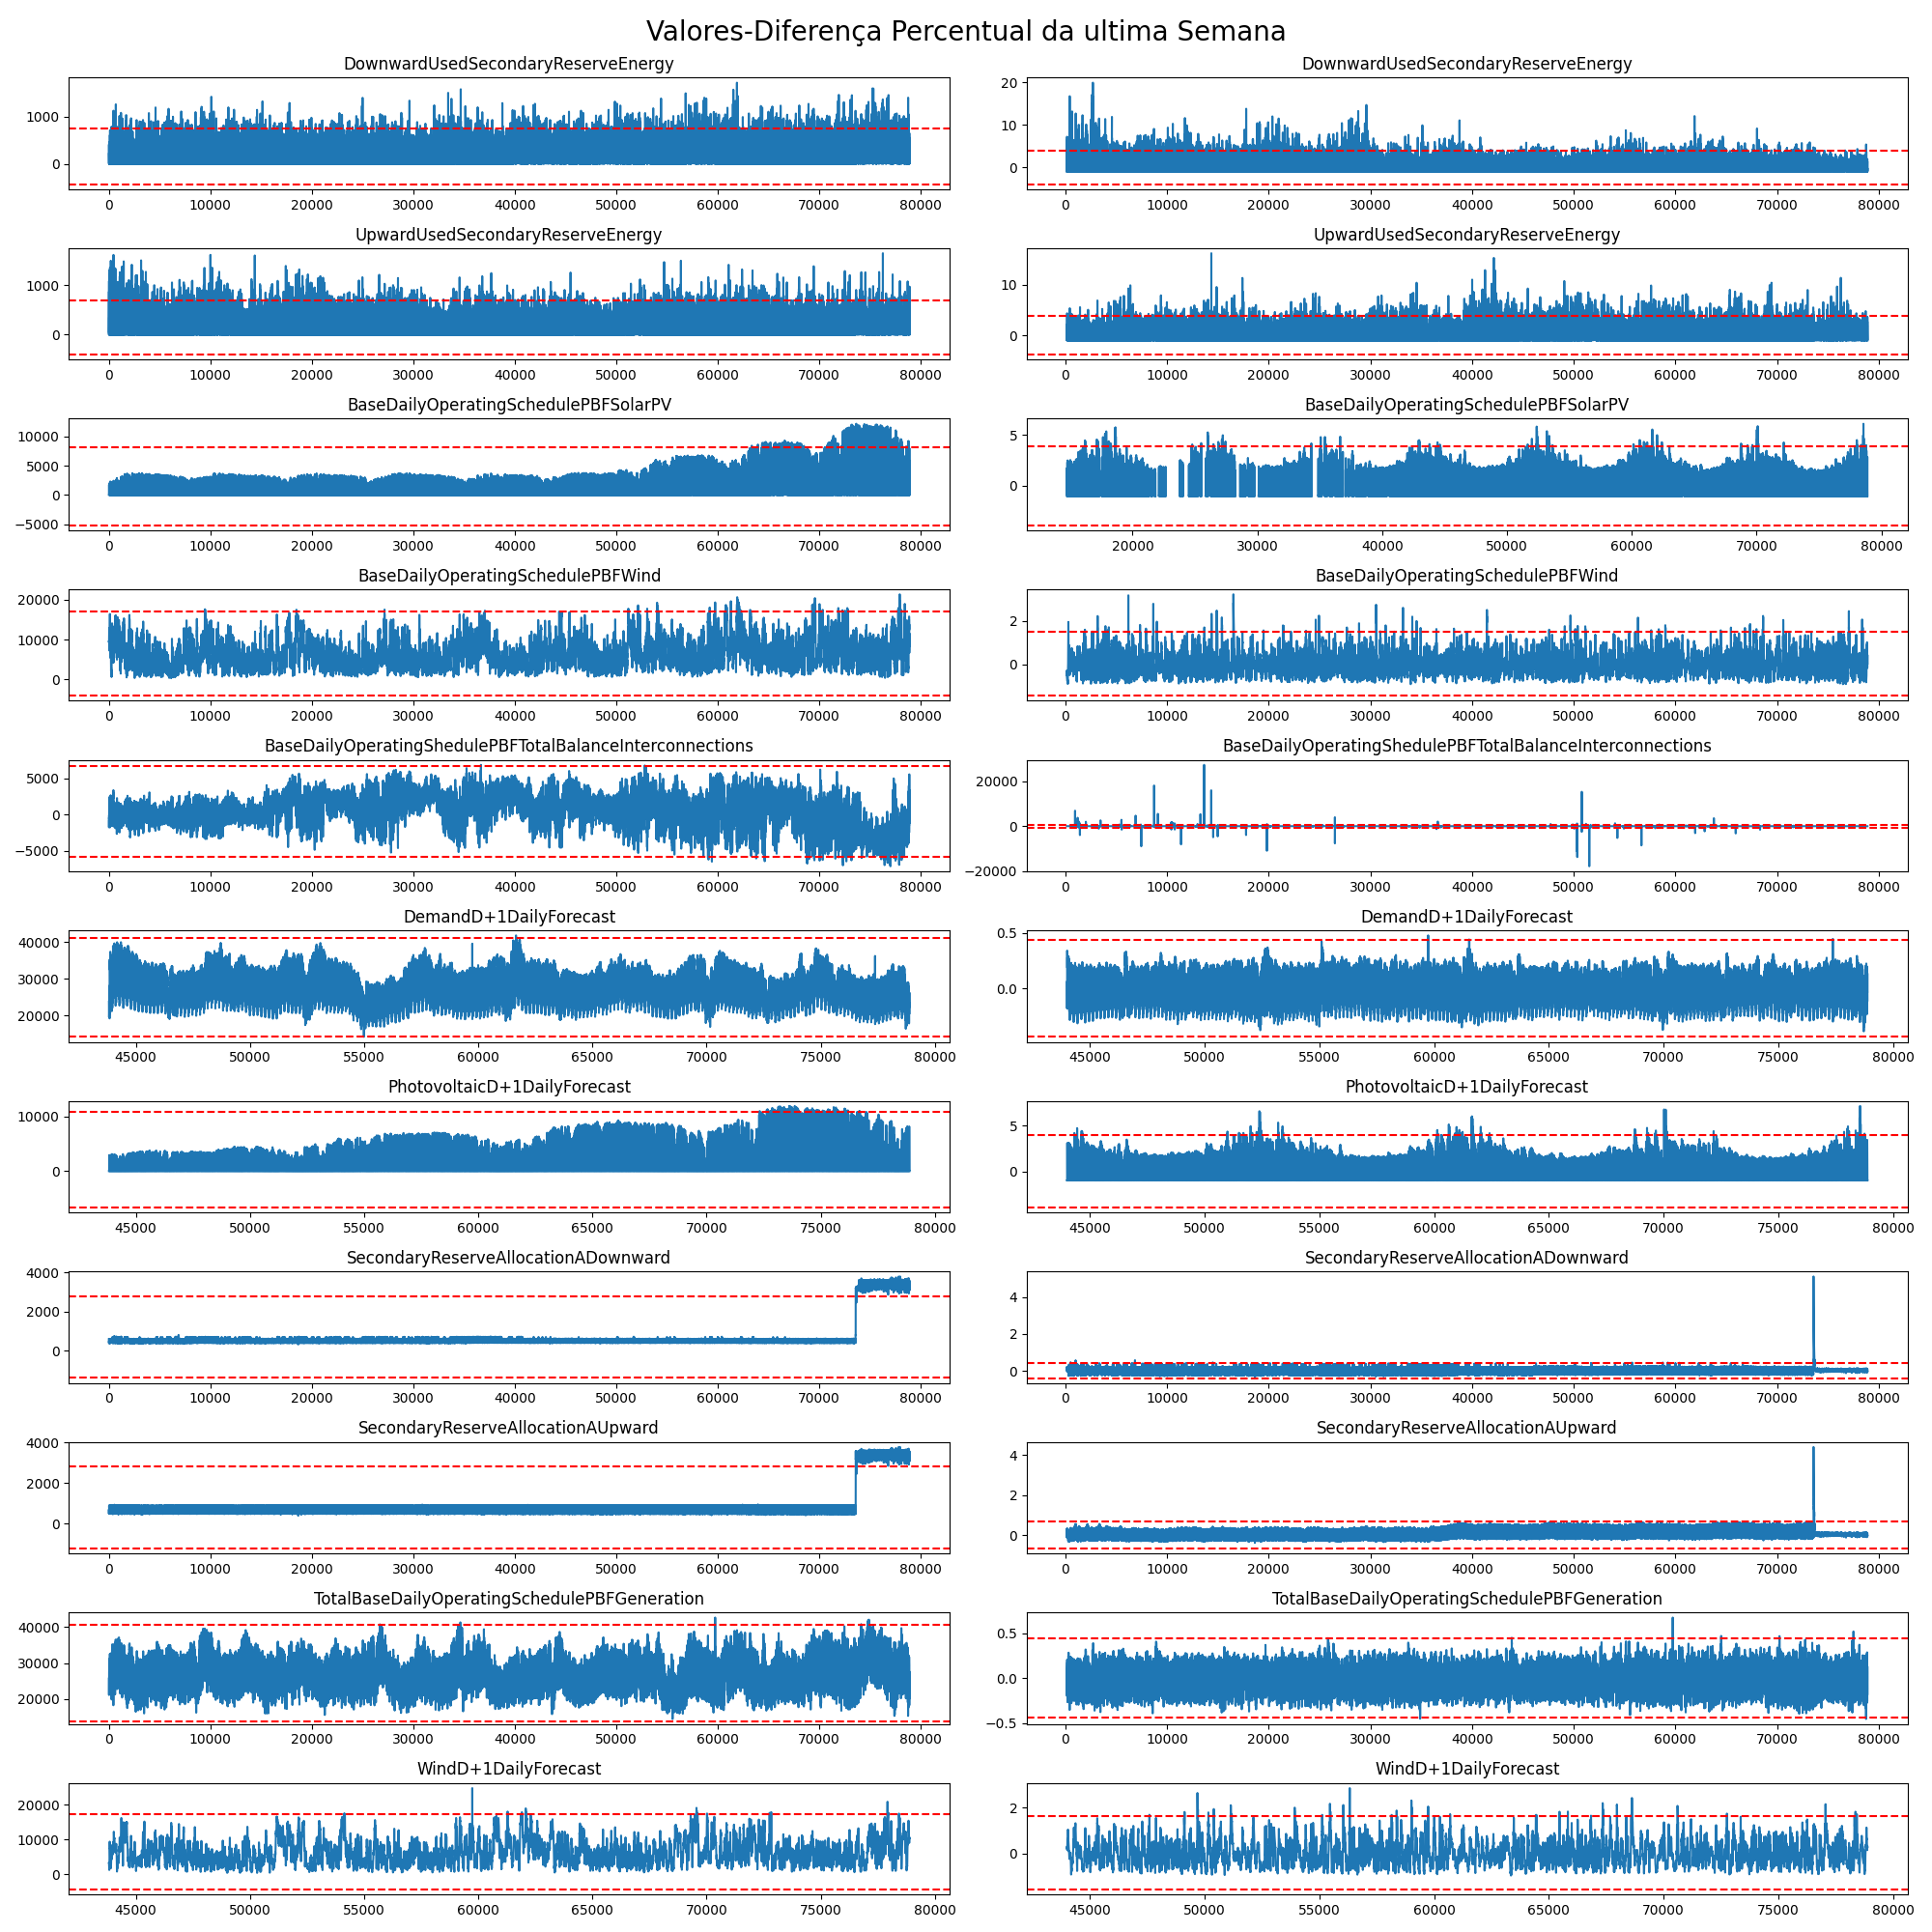
\includegraphics[width=\textwidth]{plots/Outliers_3stds.png}
  \caption{Outliers}
\end{figure}

Outra análise desta variação dos atributos a nível temporal leva-nos a que qualquer divisão dos dados para treino e teste deva levar as variações em consideração. Isto sendo que o treino deve ter representatividade de todas, ou maior parte, das condições diferentes.\par


\textbf{Dados em falta (Missing Data)}

Estudemos também o caso de dados em falta. Alguns destes atributos têm certas entradas vazias, e como podemos ver alguns não têm alguns anos inteiros.\par
Como queremos usar o máximo de dados possíveis iremos usar técnicas de imputing nesses dados.\par
Podemos ver que temos dados em falta de vários anos, em três atributos, e um tem algumas horas esporádicas em falta nos primeiros anos.\par

\begin{figure}[H]
  \centering
  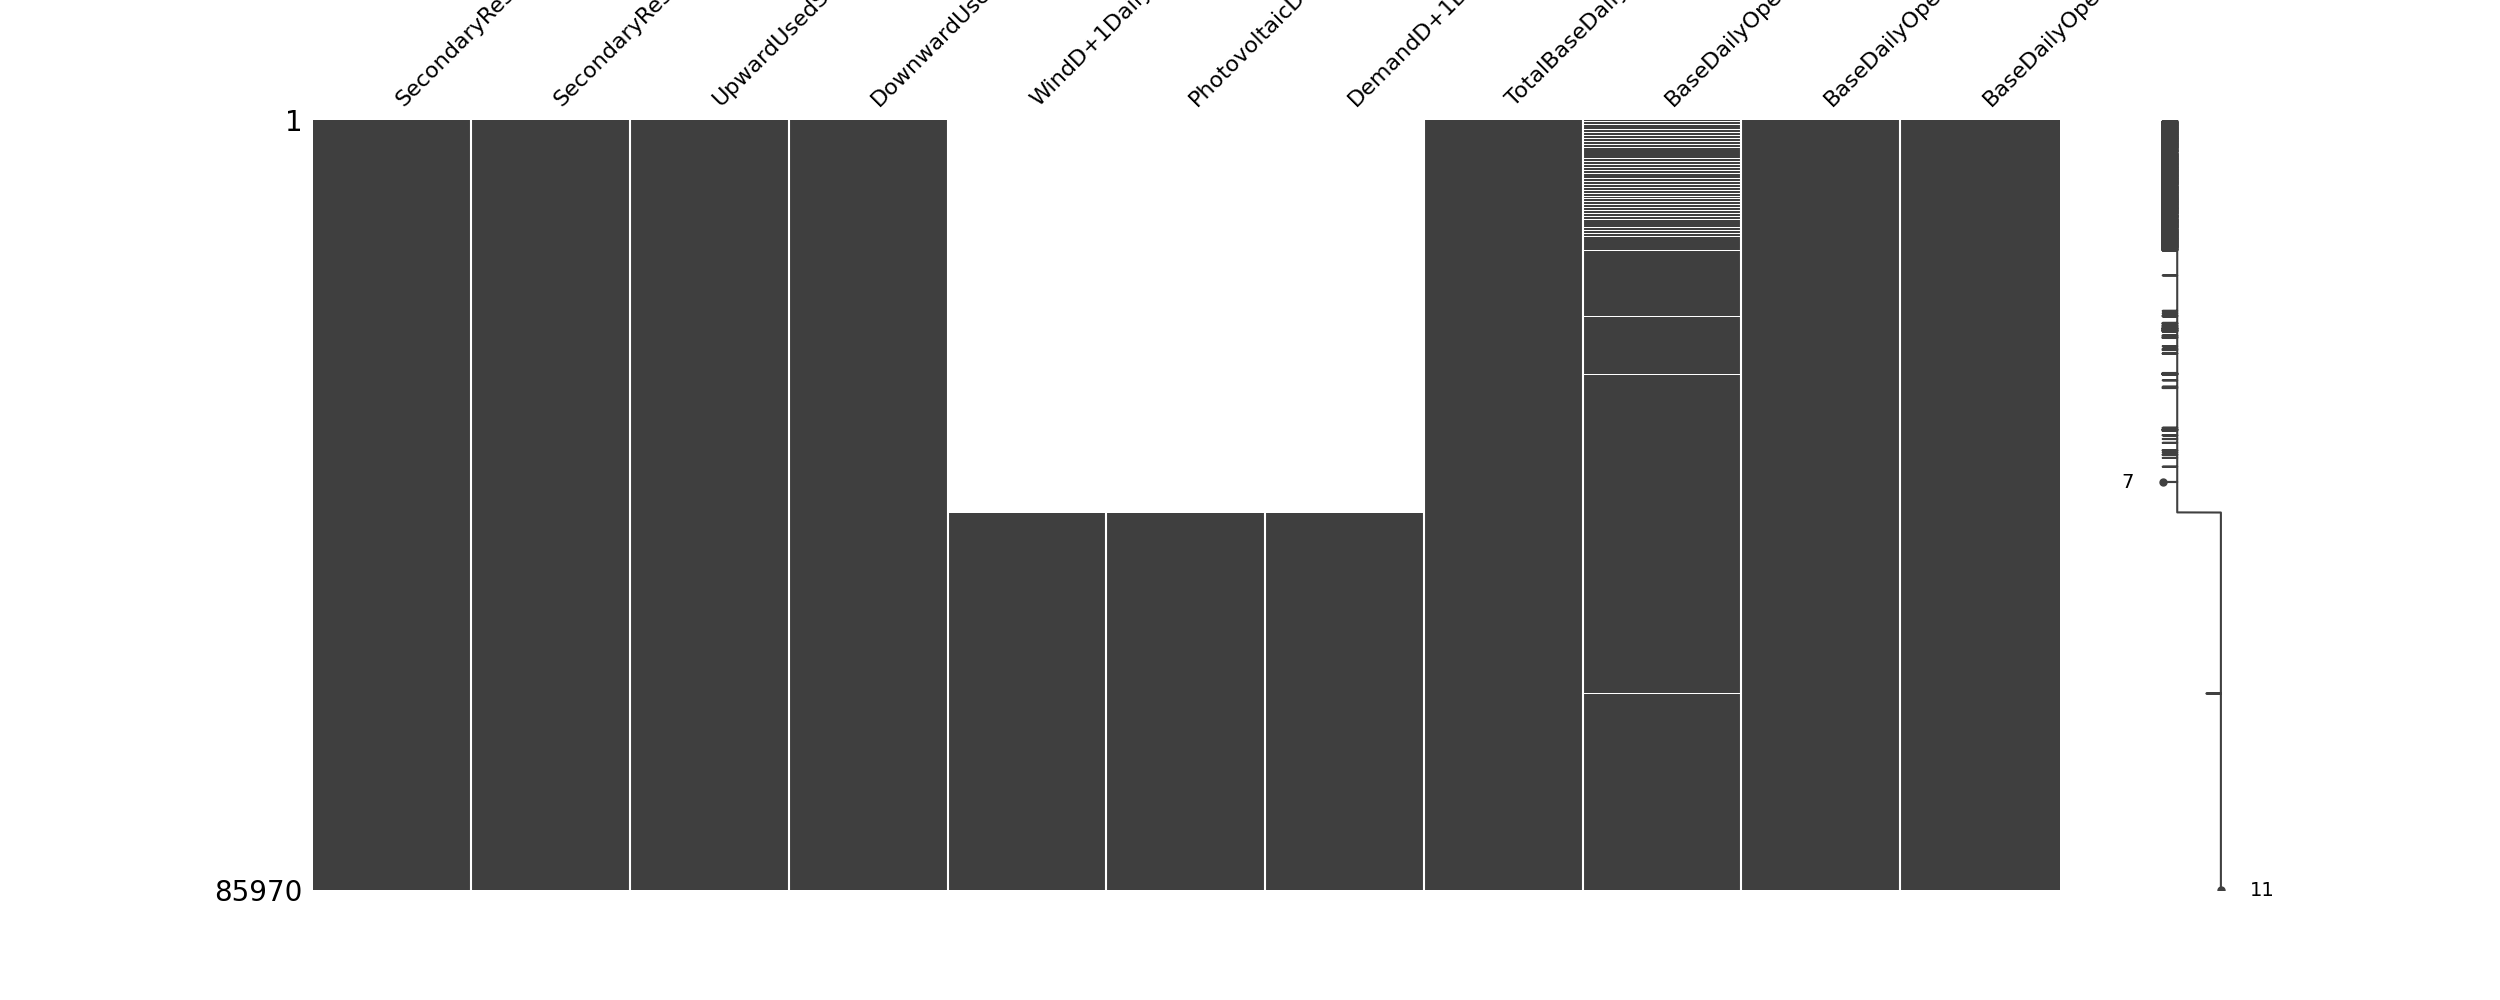
\includegraphics[width=\textwidth]{plots/missing_data.png}
  \caption{Dados em falta}
\end{figure}

Vamos aplicar o método experimental \href{https://scikit-learn.org/stable/modules/generated/sklearn.impute.IterativeImputer.html}{IterativeImputer} da biblioteca de python \href{https://scikit-learn.org/stable/index.html}{sklearn}.\par
Este metodo é baseado nos trabalhos de \cite{vanBuuren2011} e de \cite{Buck1960}.\par
Por ultimo foi adicionado ao dados mais atributos, sendo eles todos de cariz temporal. É adicionado atributos correspondentes à hora, ao dia do ano, ao dia da semana, ao dia do mês, mês, ano.\par

 \label{se:tratamentodados}

\subsection{Dados de treino}

Após o tratamento apresentado as estatísticas gerais dos dados usados para treinar o modelo são:

\begin{table}[H]
    \caption{Dados de Treino}    
    \resizebox{\linewidth}{!}{\begin{table}[H] 
    \caption{Training data summary. \label{training_data_sum}}
    \newcolumntype{C}{>{\centering\arraybackslash}X}
    \begin{tabularx}{\textwidth}{CCCCC}
    \toprule
    & \textbf{mean}	& \textbf{std}	& \textbf{min} & \textbf{max}\\
    \midrule
    Down Used & 168.20 & 199.67 & 0.00 & 1721.40 \\
    Up Allocated & 662.94 & 150.62 & 399.00 & 958.00 \\
    Down Allocated & 549.27 & 126.67 & 312.00 & 956.00 \\
    Up Used & 158.10 & 191.62 & 0.00 & 1654.80 \\
    DA Wind & 5824.12 & 3413.15 & 71.33 & 20879.30 \\
    DA PV & 1666.31 & 2719.60 & 0.00 & 14925.30 \\
    DA Demand & 27944.24 & 4479.39 & 14170.00 & 41773.00 \\
    DA Schedule Generation & 27249.43 & 4603.58 & 13470.50 & 42707.60 \\
    DA Schedule PV Generation & 1714.09 & 2815.35 & 0.00 & 16358.90 \\
    DA Schedule Wind Generation & 6525.51 & 3582.36 & 308.60 & 21619.60 \\
    DA Scheduled Tie Lines & 290.58 & 2157.11 & -7817.00 & 6858.50 \\
    \bottomrule
    \end{tabularx}
    % \noindent{\footnotesize{\textsuperscript{1} Tables may have a footer.}}
\end{table}

}
    \end{table}
